\section{Durchführung}
\label{sec:Durchführung}
Zunächst werde eine Kennlinienschar erstellt indem in geeigneten Intervallen dem Aufbau die Beschlunigungsoannung $U_B$ sowie die der Saugstrom $I_\text{S}$ entnommen wird. Dies wird für 5 verschiedene Heizströme wiederholt. Bei der Berechnung der Spannungen und Ströme sind die einzelnen Wiederstände die die einzelnen Bauteile besitzen zu beachten. Desweiteren soll der Heizstrom wie auch Spannung notiert werden.

Zur Messung des Anlaufstromkurve ist Aufbau ist wie in Abbildung \ref{eqn:Anl} zu tätigen. 
\begin{figure}
  \centering
  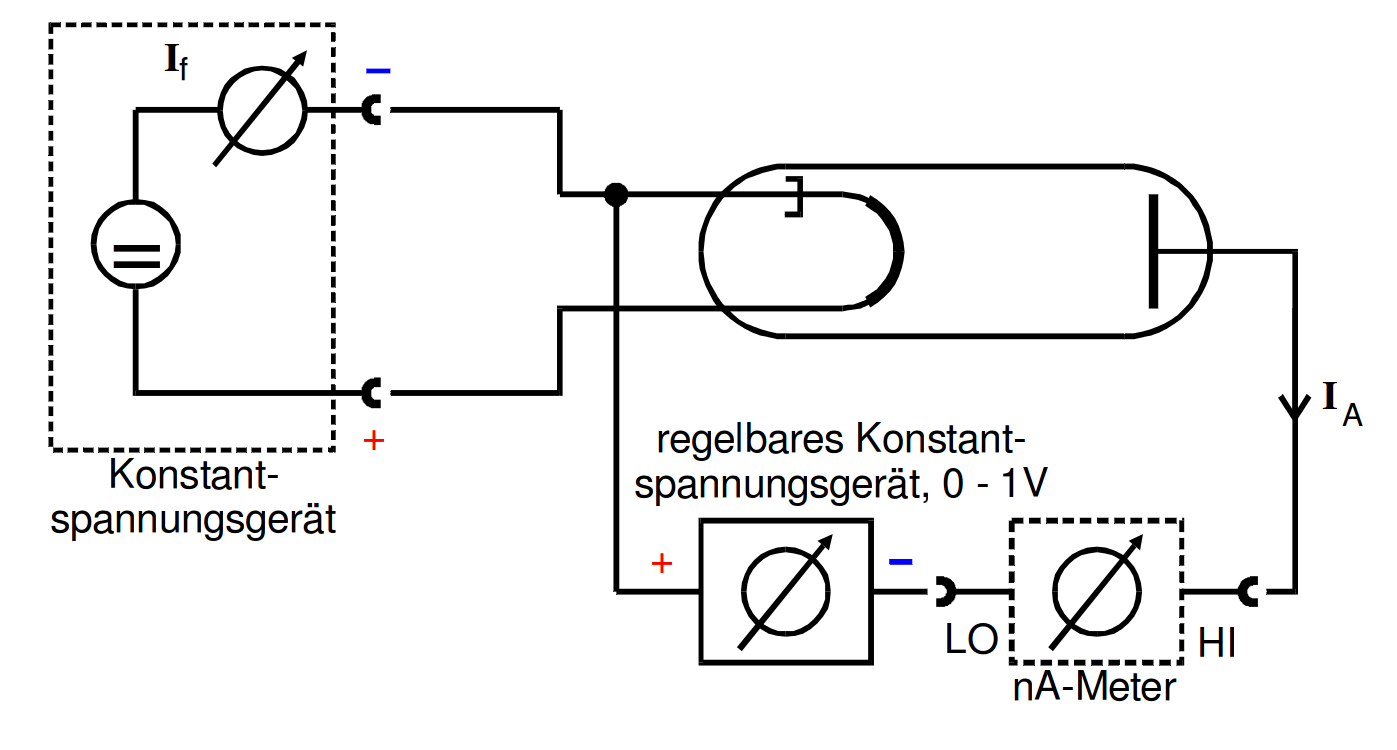
\includegraphics[height=5cm]{picture/Gegenfeld.png}
  \caption{Anlaufsstromschaltung \cite{pra}}
  \label{fig:Anl}
\end{figure}
Dabei wird in 20 äquidistanten Schritten zwischen, 0 und 1 Volt ein Gegenfeld aufgebaut. Der Heißstrom ist zu Maximieren und die Stöme im nA Bereich vom Messgerät abzulesen. Dabei ist der Wiederstand des Bananensteckers durch mehrfaches drehen zu minimieren. Zusätzlich ist darauf zu achten das durch Erschütterungen das Spannungsmessgerät nicht fälschliche Werte anzeigt. 
